\section{Linear Support Vector Regression} \label{section:svr}

In the case of regression the goal is to predict a real-valued output for $y'$ so that our training data is of the form:

\begin{equation}
	\{(x_i,y_i), x\in\Re^m, y_i\in\Re, i=1, \dots, n\} \label{eq:svr_data}
\end{equation}

The regression SVM use a loss function that not allocating a penalty if the predicted value $y'_i$ is less than a distance $\epsilon$ away from the actual value $y_i$, i.e., if $|y_i-y'_i| \leq \epsilon$, where $y'_i = w^T x_i + b$. The region bound by $y'_i\pm\epsilon \ \forall_i$ is called an $\epsilon$-insensitive tube. The output variables which are outside the tube are given one of two slack variable penalties depending on whether they lie above, $\xi^+$, or below, $\xi^-$, the tube, provided $\xi^+ \geq 0$ and $\xi^- \geq 0 \ \forall_i$:

\begin{equation} \label{eq:svr_consts}
	\begin{aligned}
		& y_i\leq y'_i+\epsilon+\xi^+ \ \forall_i \\
    	& y_i\geq y'_i-\epsilon-\xi^- \ \forall_i \\
    	& \xi_i^+, \xi_i^- \geq 0 \ \forall_i
	\end{aligned}
\end{equation}

The objective function for SVR can then be written as:

\begin{equation} \label{eq:quad_svr_obj}
    \begin{aligned}
        \min_{w,b,\xi^+,\xi^-} \quad & \frac{1}{2} \| w \|^2 + C \sum_{i=1}^n (\xi_i^+ + \xi_i^-) \\
            \text{subject to} \quad & y_i - w^T x_i - b \leq \epsilon + \xi_i^+ \ \forall_i \\ & w^T x_i + b - y_i \leq \epsilon + \xi_i^- \ \forall_i \\ & \xi_i^+, \xi_i^- \geq 0 \ \forall_i
    \end{aligned}
\end{equation}

\begin{figure}[h!]
	\centering
  	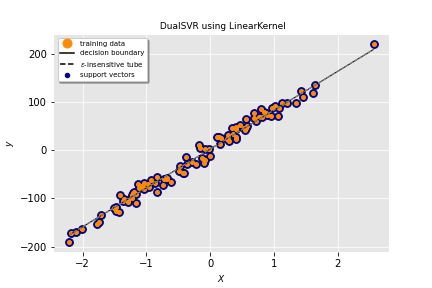
\includegraphics[scale=0.6]{img/linear_dual_l1_svr_hyperplane}
  	\caption{Linear SVR hyperplane}
  	\label{fig:linear_dual_l1_svr_hyperplane}
\end{figure}

\pagebreak

\subsection{Epsilon-insensitive loss}

The \emph{epsilon-insensitive} loss is defined as:

\begin{equation} \label{eq:eps_loss1}
	\mathcal{L}_\epsilon^1 = \max(0, |y - (w^T x + b)| - \epsilon)
\end{equation}

or, equivalently:

\begin{equation} \label{eq:eps_loss2}
	\mathcal{L}_\epsilon^1 = 
	\begin{cases}
		0 & \text{if} \ |y - (w^T x + b)| \leq \epsilon \\
		|y - (w^T x + b)| - \epsilon & \text{otherwise} \\
	\end{cases}
\end{equation}

As the \emph{hinge} loss, also the \emph{epsilon-insensitive} loss is a nondifferentiable convex function due to its nonsmoothness in $\pm\epsilon$, but has a subgradient that is given by:

% http://juliaml.github.io/LossFunctions.jl/stable/losses/distance/#L1EpsilonInsLoss-1

\begin{equation} \label{eq:eps_loss_der}
	\partial_w \mathcal{L}_\epsilon^1=
		\begin{cases}
            \displaystyle \frac{y - (w^T x + b)}{|y - (w^T x + b)|}x & \text{if} \ |y - (w^T x + b)| \geq \epsilon \\
            0 & \text{otherwise} \\ 
        \end{cases}
\end{equation}

\subsubsection{Primal formulation}

The general primal unconstrained formulation takes the same form of~\eqref{eq:primal_svm}.

The quadratic optimization problem~\eqref{eq:quad_svr_obj} can be equivalently formulated as:

\begin{equation} \label{eq:primal_l1_svr}
	\min_{w,b} \frac{1}{2} \| w \|^2 + C \sum_{i=1}^n \max(0, |y_i - (w^T x_i + b)| - \epsilon)
\end{equation}

where we make use of the \emph{epsilon-insensitive} loss~\eqref{eq:eps_loss1} or~\eqref{eq:eps_loss2}.

The above formulation penalizes slacks $\xi$ linearly and is called $\mathcal{L}_1$-SVR.

The $\mathcal{L}_1$-SVR objective~\eqref{eq:primal_l1_svr} can be rewritten in form~\eqref{eq:reg_bias_primal_svm1} or~\eqref{eq:reg_bias_primal_svm2} as:

\begin{equation} \label{eq:reg_bias_primal_l1_svr}
	\min_{w,b} \frac{1}{2} (\| w \|^2 + b^2) + C \sum_{i=1}^n \max(0, |y_i - (w^T x_i + b)| - \epsilon)
\end{equation}

\begin{figure}[h!]
	\centering
  	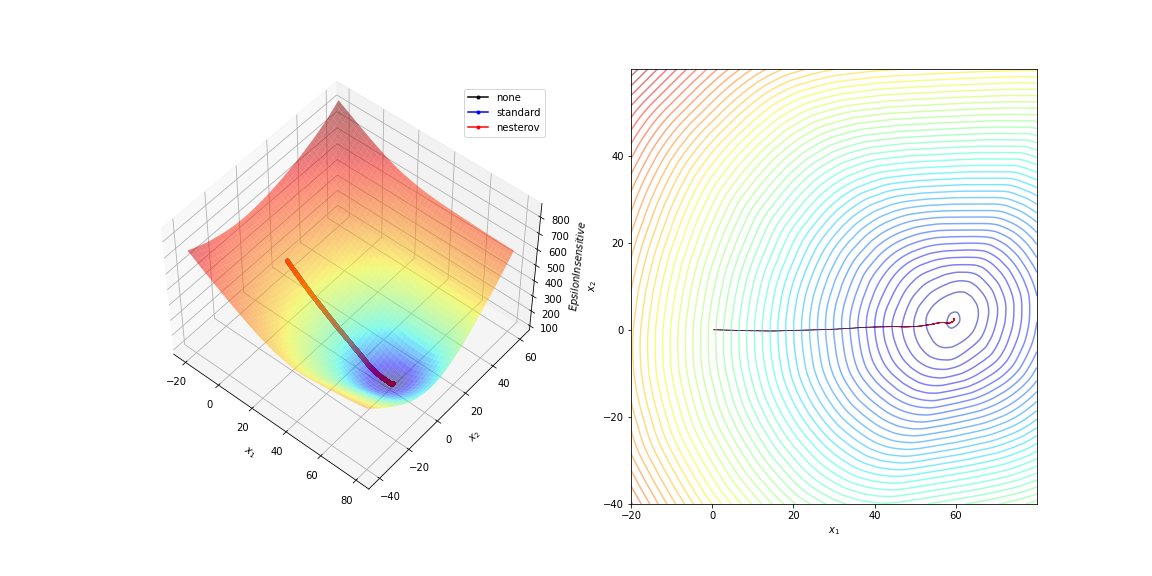
\includegraphics[scale=0.4]{img/l1_svr_loss}
  	\caption{Epsilon-insensitive loss with different optimization steps}
  	\label{fig:l1_svr_loss}
\end{figure}

\subsubsection{Wolfe dual formulation}

To reformulate the~\eqref{eq:quad_svr_obj} as a \emph{Wolfe dual}, we introduce the Lagrange multipliers $\alpha_i^+, \alpha_i^-, \mu_i^+, \mu_i^- \geq 0 \ \forall_i$:

\begin{equation} \label{eq:svr_wolfe_dual}
	\begin{aligned}
    	\max_{\alpha^+,\alpha^-,\mu^+,\mu^-} \min_{w,b,\xi^+,\xi^-} \mathcal{W}(w,b,\xi^+,\xi^-,\alpha^+,\alpha^-,\mu^+,\mu^-) = \frac{1}{2} \| w \|^2 + C \sum_{i=1}^n (\xi_i^+ + \xi_i^-)-\sum_{i=1}^n (\mu_i^+ \xi_i^+ + \mu_i^- \xi_i^-) \\ -\sum_{i=1}^n \alpha_i^+(\epsilon+\xi_i^+ + y'_i-y_i)-\sum_{i=1}^n \alpha_i^-(\epsilon+\xi_i^- - y'_i+y_i)
	\end{aligned}
\end{equation}

Substituting for $y_i$, differentiating wrt $w, b, \xi^+$, $\xi^-$ and setting the derivatives to $0$ gives:

\begin{equation} \label{eq:svr_wolfe_der_w}
	\frac{\partial \mathcal{W}}{\partial w}=w-\sum_{i=1}^n (\alpha_i^+ - \alpha_i^-) x_i \Rightarrow w=\sum_{i=1}^n (\alpha_i^+ - \alpha_i^-) x_i
\end{equation}

\begin{equation} \label{eq:svr_wolfe_der_b}
	\frac{\partial \mathcal{W}}{\partial b}=-\sum_{i=1}^n (\alpha_i^+ - \alpha_i^-)\Rightarrow \sum_{i=1}^n (\alpha_i^+ - \alpha_i^-)=0
\end{equation}

\begin{equation}\label{eq:svr_wolfe_der_xip}
	\frac{\partial \mathcal{W}}{\partial\xi_i^+}=0\Rightarrow C=\alpha_i^+ + \mu_i^+
\end{equation}

\begin{equation} \label{eq:svr_wolfe_der_xim}
	\frac{\partial \mathcal{W}}{\partial\xi_i^-}=0\Rightarrow C=\alpha_i^- + \mu_i^-
\end{equation}

Substituting~\eqref{eq:svr_wolfe_der_w} and~\eqref{eq:svr_wolfe_der_b} in, we now need to maximize $\mathcal{W}$ wrt $\alpha_i^+$ and $\alpha_i^-$, where $\alpha_i^+ \geq 0,\ \alpha_i^- \geq 0 \ \forall_i$:

\begin{equation} \label{eq:svr_max_wolfe_dual}
    \max_{\alpha^+,\alpha^-} \mathcal{W}(\alpha^+,\alpha^-) = \sum_{i=1}^n y_i(\alpha_i^+ - \alpha_i^-)-\epsilon\sum_{i=1}^n (\alpha_i^+ + \alpha_i^-)-\frac{1}{2}\sum_{i,j}(\alpha_i^+ - \alpha_i^-)\langle x_i, x_j \rangle(\alpha_j ^+ - \alpha_j ^-)
\end{equation}

Using $\mu_i^+ \geq 0$ and $\mu_i^- \geq 0$ together with~\eqref{eq:svr_wolfe_der_w} and~\eqref{eq:svr_wolfe_der_b} means that $\alpha_i^+ \leq C$ and $\alpha_i^- \leq C$. We therefore need to find:

\begin{equation} \label{eq:svr_min_wolfe_dual}
    \begin{aligned}
        \min_{\alpha^+,\alpha^-} \quad & \frac{1}{2}(\alpha^+ - \alpha^-)^TK(\alpha^+ - \alpha^-)+\epsilon e^T(\alpha^+ + \alpha^-)-y^T(\alpha^+ - \alpha^-) \\
            \text{subject to} \quad & 0\leq\alpha_i^+,\alpha_i^- \leq C \ \forall_i \\ & e^T(\alpha^+ - \alpha^-)=0
    \end{aligned}
\end{equation}

where $e^T = [1, \dots, 1]$.

We can write the~\eqref{eq:svr_min_wolfe_dual} in a standard quadratic form as:

\begin{equation}
    \begin{aligned} \label{eq:svr_min_qp_wolfe_dual}
        \min_{\alpha} \quad & \frac{1}{2}\alpha^T Q\alpha-q^T\alpha \\
            \text{subject to} \quad & 0\leq\alpha_i\leq C \ \forall_i \\ & e^T\alpha=0
    \end{aligned}
\end{equation}

where the Hessian matrix $Q =
\begin{bmatrix}
K & -K\\
-K & K 
\end{bmatrix}$
, $\alpha = 
\begin{bmatrix}
\alpha^+\\
\alpha^-
\end{bmatrix}$
, $q =
\begin{bmatrix}
-y\\
y
\end{bmatrix} + \epsilon$
, and $e =
\begin{bmatrix}
1\\
-1
\end{bmatrix}$.

Each new predictions $y'$ can be found using:

\begin{equation} \label{eq:svr_pred}
    y'= \sum_{i=1}^n (\alpha_i^+ - \alpha_i^-)\langle x_i, x' \rangle+b
\end{equation}

A set $S$ of support vectors $x_s$ can be created by finding the indices $i$ where $0\leq\alpha\leq C$ and $\xi_i^+=0$ or $\xi_i^-=0$.

This gives us:

\begin{equation} \label{eq:svr_b}
    b=y_s-\epsilon-\sum_{m\in S}(\alpha_m^+ -\alpha_m^-) \langle x_m, x_s \rangle
\end{equation}

As before it is better to average over all the indices $i$ in $S$:

\begin{equation} \label{eq:svr_b_avg}
    b=\frac{1}{N_s}\sum_{s\in S}y_s-\epsilon-\sum_{m \in S}(\alpha_m^+ - \alpha_m^-)\langle x_m, x_s \rangle
\end{equation}

From~\eqref{eq:svr_min_qp_wolfe_dual} we can notice that the equality constraint $e^T \alpha = 0$ arises form the stationarity condition $\partial_{{b}} \mathcal{W}=0$. So, again, for simplicity, we can again consider the bias term $b$ embedded into the weight vector. We report below the box-constrained dual formulation~\cite{hsu2002simple} that arises from the primal~\eqref{eq:reg_bias_primal_svm1} or~\eqref{eq:reg_bias_primal_svm2} where the bias term $b$ is embedded into the weight vector $w$:

\begin{equation} \label{eq:svr_min_bcqp_wolf_dual}
    \begin{aligned}
        \min_{\alpha} \quad & \frac{1}{2} \alpha^T (Q + ee^T)\alpha+q^T\alpha \\
            \text{subject to} \quad & 0\leq\alpha_i\leq C \ \forall_i
    \end{aligned}
\end{equation}

\subsubsection{Lagrangian dual formulation}

In order to relax the constraints in the \emph{Wolfe dual} formulation~\eqref{eq:svr_min_wolfe_dual} we define the problem as a \emph{Lagrangian dual} relaxation by embedding them into objective function, so we need to allocate the Lagrange multipliers $\mu$ and $\lambda_+, \lambda_- \geq 0$:

\begin{equation} \label{eq:l1_svr_lagrangian_dual}
	\begin{aligned}
		    \max_{\mu,\lambda_+,\lambda_-} \min_{\alpha} \mathcal{L}(\alpha,\mu,\lambda_+,\lambda_-) &= \frac{1}{2} \alpha^T Q\alpha+q^T\alpha + \mu^T (e^T \alpha) + \lambda_+^T (ub - \alpha) - \lambda_-^T \alpha \\
    &= \frac{1}{2} \alpha^T Q\alpha + (q + \mu e^T + \lambda_+ - \lambda_-)^T \alpha + \lambda_+^T ub \\
    \text{subject to} \quad & \,\, \lambda_+, \lambda_- \geq 0
	\end{aligned}
\end{equation}

where the upper bound $ub^T = [C, \dots, C]$.

Taking the derivative of the Lagrangian $\mathcal{L}$ wrt $\alpha$ and settings it to 0 gives:

\begin{equation} \label{eq:svr_lagrangian_der_a}
	\frac{\partial \mathcal{L}}{\partial \alpha}=0\Rightarrow Q \alpha + (q + \mu e^T + \lambda_+ - \lambda_-) = 0
\end{equation}

With $\alpha$ optimal solution of the linear system:

\begin{equation} \label{eq:l1_svr_lagrangian_sol}
    Q \alpha = - (q + \mu e^T + \lambda_+ - \lambda_-)
\end{equation}

the gradients wrt $\mu$, $\lambda_+$ and $\lambda_-$ are:

\begin{equation} \label{eq:svr_lagrangian_der_mu}
	\frac{\partial \mathcal{L}}{\partial \mu}=-e \alpha
\end{equation}

\begin{equation} \label{eq:svr_lagrangian_der_lp}
	\frac{\partial \mathcal{L}}{\partial \lambda_+}=\alpha - ub
\end{equation}

\begin{equation} \label{eq:svr_lagrangian_der_lm}
    \frac{\partial \mathcal{L}}{\partial \lambda_-}=-\alpha
\end{equation}

From~\eqref{eq:svr_min_qp_wolfe_dual} we can notice that the equality constraint $e^T \alpha = 0$ arises form the stationarity condition $\partial_{{b}} \mathcal{W}=0$. So, again, for simplicity, we can again consider the bias term $b$ embedded into the weight vector. In this way the dimensionality of~\eqref{eq:l1_svr_lagrangian_dual} is reduced by removing the multipliers $\mu$ which was allocated to control the equality constraint $e^T \alpha=0$, so we will end up solving exactly the problem~\eqref{eq:svr_min_bcqp_wolf_dual}.

\begin{equation} \label{eq:l1_svr_bcqp_lagrangian_dual}
	\begin{aligned}
    	\max_{\lambda_+,\lambda_-} \min_{\alpha} \mathcal{L}(\alpha,\lambda_+,\lambda_-) &= \frac{1}{2} \alpha^T (Q + ee^T)\alpha+q^T\alpha + \lambda_+^T (ub - \alpha) - \lambda_-^T \alpha \\
    &= \frac{1}{2} \alpha^T (Q + ee^T)\alpha + (q + \lambda_+ - \lambda_-)^T \alpha + \lambda_+^T ub \\
    \text{subject to} \quad & \,\, \lambda_+, \lambda_- \geq 0
	\end{aligned}
\end{equation}

where, again, the upper bound $ub^T = [C, \dots, C]$.

Now, taking the derivative of the Lagrangian $\mathcal{L}$ wrt $\alpha$ and settings it to 0 gives:

\begin{equation} \label{eq:l1_svr_bcqp_lagrangian_der_a}
	\frac{\partial \mathcal{L}}{\partial \alpha}=0\Rightarrow (Q + ee^T) \alpha + (q + \lambda_+ - \lambda_-) = 0
\end{equation}

With $\alpha$ optimal solution of the linear system:

\begin{equation} \label{eq:l1_svr_bcqp_lagrangian_sol}
    (Q + ee^T) \alpha = - (q + \lambda_+ - \lambda_-)
\end{equation}

the gradients wrt $\lambda_+$ and $\lambda_-$ are:

\begin{equation} \label{eq:l1_svr_bcqp_lagrangian_der_lp}
	\frac{\partial \mathcal{L}}{\partial \lambda_+}=\alpha - ub
\end{equation}

\begin{equation} \label{eq:l1_svr_bcqp_lagrangian_der_lm}
    \frac{\partial \mathcal{L}}{\partial \lambda_-}=-\alpha
\end{equation}

\bigskip

Note that since the Hessian matrix $Q$ of the $\mathcal{L}_1$-SVR is not strictly positive definite, i.e., the Lagrangian function is not strictly convex since it will be linear along the eigenvectors correspondent to the null eigenvalues and so it will be unbounded below, the Lagrangian dual relaxation, i.e.,~\ref{eq:l1_svr_lagrangian_sol} and~\ref{eq:l1_svr_bcqp_lagrangian_sol}, will be nondifferentiable, so it will have infinite solutions and for each of them it will have a different subgradient. In order to compute an approximation of the gradient, we will choose $\alpha$ in such a way as the one that minimizes the 2-norm since it is good almost like the gradient:

\begin{equation} \label{eq:svr_lagrangian_krylov_sol}
	\min_{\alpha_n \in K_n(Q, b)} \| Q \alpha_n - b \|
\end{equation}

Since we are dealing with a symmetric system we will choose a well-known Krylov method that performs the Lanczos iterate, i.e., symmetric Arnoldi iterate, called \emph{minres}, i.e., symmetric \emph{gmres}, to compute the vector $\alpha_n$ that minimizes the norm of the residual $r_n = Q \alpha_n - b$ among all vectors in $K_n(Q, b) = span(b, Qb, Q^2b, \dots, Q^{n-1}b)$.

\bigskip

Since the linear algebra methods in the ML context are crucial and also in order to deal with a per-iteration cost equals to the other algorithms described later to provide a coherent comparison of all at the end, we will solve it with a primal-dual optimization method and we modify its definition by adding a strictly convex augmentation term, i.e., a penalty term, in order to improve the actual convergence of the algorithms. So, if we consider a general quadratic optimization problem subject to linear constraints, i.e., equality and inequality constraints, defined as:

\begin{equation}
    \begin{aligned} 
        \min_{\alpha} \quad & \frac{1}{2} \alpha^T Q \alpha + q^T \alpha \\
            \textrm{subject to} \quad & A \alpha = b \\ & G \alpha \leq h \\ & lb \leq \alpha \leq ub
    \end{aligned}
\end{equation}

or, equivalently:

\begin{equation}
    \begin{aligned}
        \min_{\alpha} \quad & \frac{1}{2} \alpha^T Q \alpha + q^T \alpha \\
            \textrm{subject to} \quad & A \alpha = b \\ & \hat{G} \alpha \leq \hat{h}
    \end{aligned}
\end{equation}

where $\hat{G} =
\begin{bmatrix}
 G \\
-I \\
 I 
\end{bmatrix}$ and $\hat{h} =
\begin{bmatrix}
h & -lb & ub
\end{bmatrix}$; we give the following \emph{augmented Lagrangian dual}:

\begin{equation} \label{eq:l1_svr_gen_aug_lagrangian_dual}
	\begin{aligned}
		    \max_{\mu,\lambda} \min_{\alpha} \quad & \frac{1}{2} \alpha^T Q \alpha + q^T \alpha + \mu^T (A \alpha - b) + \lambda^T (\hat{G} \alpha - \hat{h}) + \frac{\rho}{2} \| A \alpha - b \|^2 + \frac{\rho}{2} \| \hat{G} \alpha - \hat{h} \|^2 \\
    \text{subject to} \quad & \lambda \geq 0
	\end{aligned}
\end{equation}

with $\rho > 0$.

\bigskip

According to this definition, we change the formulation~\ref{eq:l1_svr_lagrangian_dual} as:

\begin{equation} \label{eq:l1_svr_aug_lagrangian_dual}
	\begin{aligned}
		    \max_{\mu,\lambda} \min_{\alpha} \mathcal{L}(\alpha,\mu,\lambda) &= \frac{1}{2} \alpha^T Q\alpha+q^T\alpha + \mu^T (e^T \alpha) + \lambda^T (\hat{G} \alpha - \hat{h}) + \frac{\rho}{2} \| e^T \alpha \|^2 + \frac{\rho}{2} \| \hat{G} \alpha - \hat{h} \|^2 \\
    \text{subject to} \quad & \,\, \lambda \geq 0
	\end{aligned}
\end{equation}

and the formulation~\ref{eq:l1_svr_bcqp_lagrangian_dual} as:

\begin{equation} \label{eq:l1_svr_bcqp_aug_lagrangian_dual}
	\begin{aligned}
    	\max_{\lambda} \min_{\alpha} \mathcal{L}(\alpha,\lambda) &= \frac{1}{2} \alpha^T (Q + ee^T) \alpha + q^T \alpha + \lambda^T (\hat{G} \alpha - \hat{h}) + \frac{\rho}{2} \| \hat{G} \alpha - \hat{h} \|^2 \\
    \text{subject to} \quad & \,\, \lambda \geq 0
	\end{aligned}
\end{equation}

where $\hat{G} =
\begin{bmatrix}
-I \\
 I 
\end{bmatrix}$ and $\hat{h} =
\begin{bmatrix}
-lb & ub
\end{bmatrix}$ with $lb^T = [0, \dots, 0]$, $ub^T = [C, \dots, C]$ and $\rho > 0$.

\pagebreak

\subsection{Squared epsilon-insensitive loss}

The \emph{squared epsilon-insensitive} loss is defined as:

\begin{equation} \label{eq:squared_eps_loss1}
	\mathcal{L}_\epsilon^2 = \max(0, |y - (w^T x + b)| - \epsilon)^2
\end{equation}

or, equivalently:

\begin{equation} \label{eq:squared_eps_loss2}
	\mathcal{L}_\epsilon^2 = 
	\begin{cases}
		0 & \text{if} \ |y - (w^T x + b)| \leq \epsilon \\
		(|y - (w^T x + b)| - \epsilon)^2 & \text{otherwise} \\
	\end{cases}
\end{equation}

As the \emph{squared hinge} loss, also the \emph{squared epsilon-insensitive} loss is a strictly convex function and its gradient is given by:

% http://juliaml.github.io/LossFunctions.jl/stable/losses/distance/#L2EpsilonInsLoss-1

\begin{equation} \label{eq:squared_eps_loss_der}
	\nabla_w \mathcal{L}_\epsilon^2=
		\begin{cases}
            \displaystyle 2 \operatorname{sign}(y - (w^T x + b)) (|y - (w^T x + b)| - \epsilon) x & \text{if} \ |y - (w^T x + b)| \geq \epsilon \\
            0 & \text{otherwise} \\ 
        \end{cases}
\end{equation}

\subsubsection{Primal formulation}

To provide a continuously differentiable function the optimization problem~\eqref{eq:primal_l1_svr} can be formulated as:

\begin{equation} \label{eq:primal_l2_svr}
    \min_{w,b} \frac{1}{2} \| w \|^2 + C \sum_{i=1}^n \max(0, |y_i - (w^T x_i + b)| - \epsilon)^2
\end{equation}

where we make use of the \emph{squared epsilon-insensitive} loss that quadratically penalized slacks $\xi$ and is called $\mathcal{L}_2$-SVR.

The $\mathcal{L}_2$-SVR objective~\eqref{eq:primal_l2_svr} can be rewritten in form~\eqref{eq:reg_bias_primal_svm1} or~\eqref{eq:reg_bias_primal_svm2} as:

\begin{equation} \label{eq:reg_bias_primal_l2_svr}
	\min_{w,b} \frac{1}{2} (\| w \|^2 + b^2) + C \sum_{i=1}^n \max(0, |y_i - (w^T x_i + b)| - \epsilon)^2
\end{equation}

\begin{figure}[h!]
	\centering
  	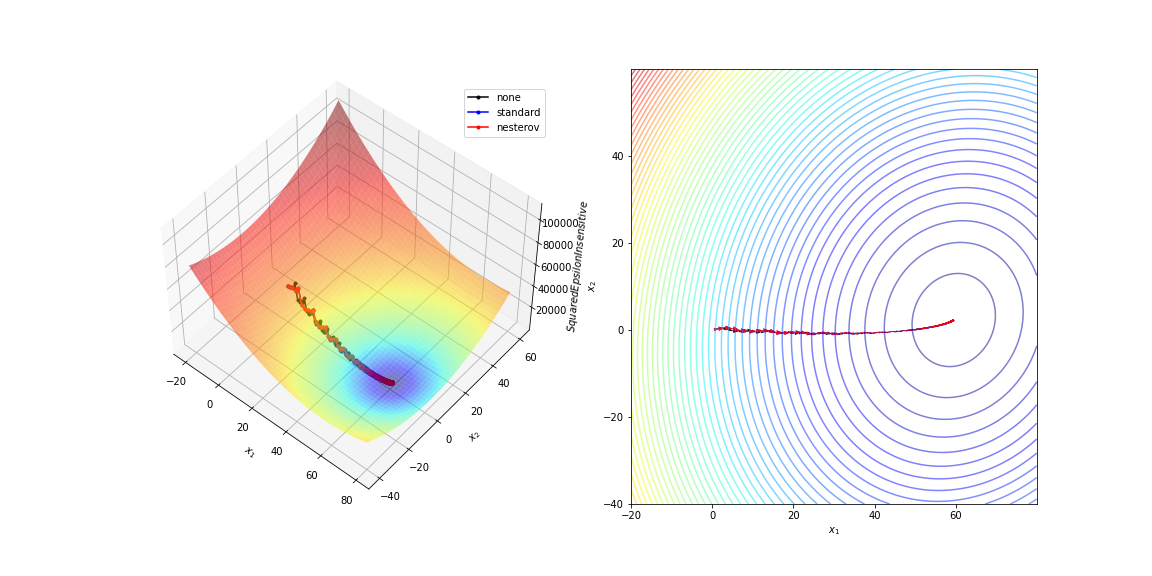
\includegraphics[scale=0.4]{img/l2_svr_loss}
  	\caption{Squared epsilon-insensitive loss with different optimization steps}
  	\label{fig:l2_svr_loss}
\end{figure}

\subsubsection{Wolfe dual formulation}

As done for the $\mathcal{L}_1$-SVR we can derive the \emph{Wolfe dual} formulation of the $\mathcal{L}_2$-SVR by obtaining:

\begin{equation} \label{eq:wolfe_dual_l2_svr}
    \begin{aligned}
        \min_{\alpha} \quad & \frac{1}{2} \alpha^T (Q + D) \alpha + q^T \alpha \\
            \text{subject to} \quad & \alpha_i \geq 0 \ \forall_i \\ & e^T \alpha=0
    \end{aligned}
\end{equation}

or, alternatively, with the regularized bias term by obtaining:

\begin{equation} \label{eq:reg_bias_wolfe_dual_l2_svr}
    \begin{aligned}
        \min_{\alpha} \quad & \frac{1}{2}\alpha^T (Q + ee^T + D) \alpha + q^T \alpha \\
            \text{subject to} \quad & \alpha_i \geq 0 \ \forall_i
    \end{aligned}
\end{equation}

where the diagonal matrix $\displaystyle D_{ii} = \frac{1}{2C} \ \forall_i$.

\subsubsection{Lagrangian dual formulation}

In order to relax the constraints in the $\mathcal{L}_2$-SVR \emph{Wolfe dual} formulation~\eqref{eq:wolfe_dual_l2_svr} we define the problem as a \emph{Lagrangian dual} relaxation by embedding them into objective function, so we need to allocate the Lagrange multipliers $\mu$ and $\lambda \geq 0$:

\begin{equation} \label{eq:l2_svr_lagrangian_dual}
	\begin{aligned}
		    \max_{\mu,\lambda} \min_{\alpha} \mathcal{L}(\alpha,\mu,\lambda) &= \frac{1}{2} \alpha^T (Q+D)\alpha+q^T\alpha + \mu^T (e^T \alpha) - \lambda^T \alpha \\
    &= \frac{1}{2} \alpha^T (Q+D)\alpha + (q + \mu e^T - \lambda)^T \alpha \\
    \text{subject to} \quad & \,\, \lambda \geq 0
	\end{aligned}
\end{equation}

Taking the derivative of the Lagrangian $\mathcal{L}$ wrt $\alpha$ and settings it to 0 gives:

\begin{equation} \label{eq:l2_svr_lagrangian_der_a}
	\frac{\partial \mathcal{L}}{\partial \alpha}=0\Rightarrow (Q+D) \alpha + (q + \mu e^T - \lambda) = 0
\end{equation}

With $\alpha$ optimal solution of the linear system:

\begin{equation} \label{eq:l2_svr_lagrangian_sol}
    (Q+D) \alpha = - (q + \mu e^T - \lambda)
\end{equation}

the gradients wrt $\mu$ and $\lambda$ are:

\begin{equation} \label{eq:l2_svr_lagrangian_der_mu}
	\frac{\partial \mathcal{L}}{\partial \mu}=-e \alpha
\end{equation}

\begin{equation} \label{eq:l2_svr_lagrangian_der_lalbda}
    \frac{\partial \mathcal{L}}{\partial \lambda}=-\alpha
\end{equation}

From~\eqref{eq:svr_min_qp_wolfe_dual} we can notice that the equality constraint $e^T \alpha = 0$ arises form the stationarity condition $\partial_{{b}} \mathcal{W}=0$. So, again, for simplicity, we can again consider the bias term $b$ embedded into the weight vector. In this way the dimensionality of~\eqref{eq:l2_svr_lagrangian_dual} is reduced by removing the multipliers $\mu$ which was allocated to control the equality constraint $e^T \alpha=0$, so we will end up solving exactly the problem~\eqref{eq:reg_bias_wolfe_dual_l2_svr}.

\begin{equation} \label{eq:l2_svr_lb_lagrangian_dual}
	\begin{aligned}
    	\max_{\lambda} \min_{\alpha} \mathcal{L}(\alpha,\lambda) &= \frac{1}{2} \alpha^T (Q + ee^T + D) \alpha+q^T\alpha - \lambda^T \alpha \\
    &= \frac{1}{2} \alpha^T (Q + ee^T + D)\alpha + (q - \lambda)^T \alpha \\
    \text{subject to} \quad & \,\, \lambda \geq 0
	\end{aligned}
\end{equation}

Now, taking the derivative of the Lagrangian $\mathcal{L}$ wrt $\alpha$ and settings it to 0 gives:

\begin{equation} \label{eq:l2_svr_lb_lagrangian_der_a}
	\frac{\partial \mathcal{L}}{\partial \alpha}=0\Rightarrow (Q + ee^T + D) \alpha + (q - \lambda) = 0
\end{equation}

With $\alpha$ optimal solution of the linear system:

\begin{equation} \label{eq:l2_svr_lb_lagrangian_sol}
    (Q + ee^T + D) \alpha = - (q - \lambda)
\end{equation}

the gradient wrt $\lambda$ is:

\begin{equation} \label{eq:l2_svr_lb_lagrangian_der_l}
    \frac{\partial \mathcal{L}}{\partial \lambda}=-\alpha
\end{equation}

\bigskip

Note that since the Hessian matrix $Q$ of the $\mathcal{L}_2$-SVR is symmetric and strictly positive definite, we can find the unique solution of the Lagrangian dual relaxation, i.e.,~\ref{eq:l2_svr_lagrangian_sol} and~\ref{eq:l2_svr_lb_lagrangian_sol}, by solving the system with the Cholesky factorization.

\bigskip

Since the linear algebra methods in the ML context are crucial and also in order to deal with a per-iteration cost equals to the other algorithms described later to provide a coherent comparison of all at the end, we will solve it with a primal-dual optimization method and we modify its definition by adding a strictly convex augmentation term, i.e., a penalty term, in order to improve the actual convergence of the algorithms. So, if we consider a general quadratic optimization problem subject to linear constraints, i.e., equality and inequality constraints, defined as:

\begin{equation}
    \begin{aligned} 
        \min_{\alpha} \quad & \frac{1}{2} \alpha^T Q \alpha + q^T \alpha \\
            \textrm{subject to} \quad & A \alpha = b \\ & G \alpha \leq h \\ & lb \leq \alpha \leq ub
    \end{aligned}
\end{equation}

or, equivalently:

\begin{equation}
    \begin{aligned}
        \min_{\alpha} \quad & \frac{1}{2} \alpha^T Q \alpha + q^T \alpha \\
            \textrm{subject to} \quad & A \alpha = b \\ & \hat{G} \alpha \leq \hat{h}
    \end{aligned}
\end{equation}

where $\hat{G} =
\begin{bmatrix}
 G \\
-I \\
 I 
\end{bmatrix}$ and $\hat{h} =
\begin{bmatrix}
h & -lb & ub
\end{bmatrix}$; we give the following \emph{augmented Lagrangian dual}:

\begin{equation} \label{eq:l2_svr_gen_aug_lagrangian_dual}
	\begin{aligned}
		    \max_{\mu,\lambda} \min_{\alpha} \quad & \frac{1}{2} \alpha^T Q \alpha + q^T \alpha + \mu^T (A \alpha - b) + \lambda^T (\hat{G} \alpha - \hat{h}) + \frac{\rho}{2} \| A \alpha - b \|^2 + \frac{\rho}{2} \| \hat{G} \alpha - \hat{h} \|^2 \\
    \text{subject to} \quad & \lambda \geq 0
	\end{aligned}
\end{equation}

with $\rho > 0$.

\bigskip

According to this definition, we change the formulation~\ref{eq:l2_svr_lagrangian_dual} as:

\begin{equation} \label{eq:l2_svr_aug_lagrangian_dual}
	\begin{aligned}
		    \max_{\mu,\lambda} \min_{\alpha} \mathcal{L}(\alpha,\mu,\lambda) &= \frac{1}{2} \alpha^T (Q + D) \alpha+q^T\alpha + \mu^T (e^T \alpha) + \lambda^T (\hat{G} \alpha - \hat{h}) + \frac{\rho}{2} \| e^T \alpha \|^2 + \frac{\rho}{2} \| \hat{G} \alpha - \hat{h} \|^2 \\
    \text{subject to} \quad & \,\, \lambda \geq 0
	\end{aligned}
\end{equation}

and the formulation~\ref{eq:l2_svr_lb_lagrangian_dual} as:

\begin{equation} \label{eq:l2_svr_lb_aug_lagrangian_dual}
	\begin{aligned}
    	\max_{\lambda} \min_{\alpha} \mathcal{L}(\alpha,\lambda) &= \frac{1}{2} \alpha^T (Q + ee^T + D) \alpha + q^T \alpha + \lambda^T (\hat{G} \alpha - \hat{h}) + \frac{\rho}{2} \| \hat{G} \alpha - \hat{h} \|^2 \\
    \text{subject to} \quad & \,\, \lambda \geq 0
	\end{aligned}
\end{equation}

where $\hat{G} =
\begin{bmatrix}
-I
\end{bmatrix}$ and $\hat{h} =
\begin{bmatrix}
-lb
\end{bmatrix}$ with $lb^T = [0, \dots, 0]$ and $\rho > 0$.